
	
	
\section{KDE Architecture}
Im Folgenden wird nun die Architektur der vom Team des KDE Projekts entwickelten KDE Software Compilation (KDE SC) vorgestellt. Der wohl bekannteste Teil der KDE Software Compilation ist die Desktop Umgebung KDE Plasma. Dazu kommt eine große Anzahl an Anwendungen die KDE Applications. Diese werden vor allem in Verbindung mit KDE Plasma genutzt können aber auch unabhängig davon verwendet werden. Der dritte Bestandteil der KDE Software Compilation heißt KDE Frameworks und stellt eine Sammlung von Bibliotheken dar. Diese enthalten häufig benötigte Funktionen und machen es somit einfacher KDE Software zu entwickeln. Außerdem wird so das ständige neu entwickeln grundlegender Funktionen verhindert. Wichtig ist in diesem Zusammenhang auch die Qt Library die zwar nicht direkt zum KDE Projekt gehört aber eng mit dem KDE Projekt verbunden ist da Qt als Basis für die Entwicklung verwendet wird.
Qt (http://www.qt.io/) ist im wesentlichen eine C++-Klassenbibliothek für die plattformübergreifende Programmierung grafischer Benutzeroberflächen die viele für die Entwicklung hilfreiche Funktionen bietet.
%\url{https://en.wikipedia.org/wiki/Qt_(software)}
%\url{http://www.qt.io/}
Auf Anwenderebene sind also die KDE Applications und KDE Plasma die auf die KDE Framworks und Qt aufbauen wie auch in Abbildung \ref{fig:kde_overview} dargestellt.
\begin{figure}[h]
\centering
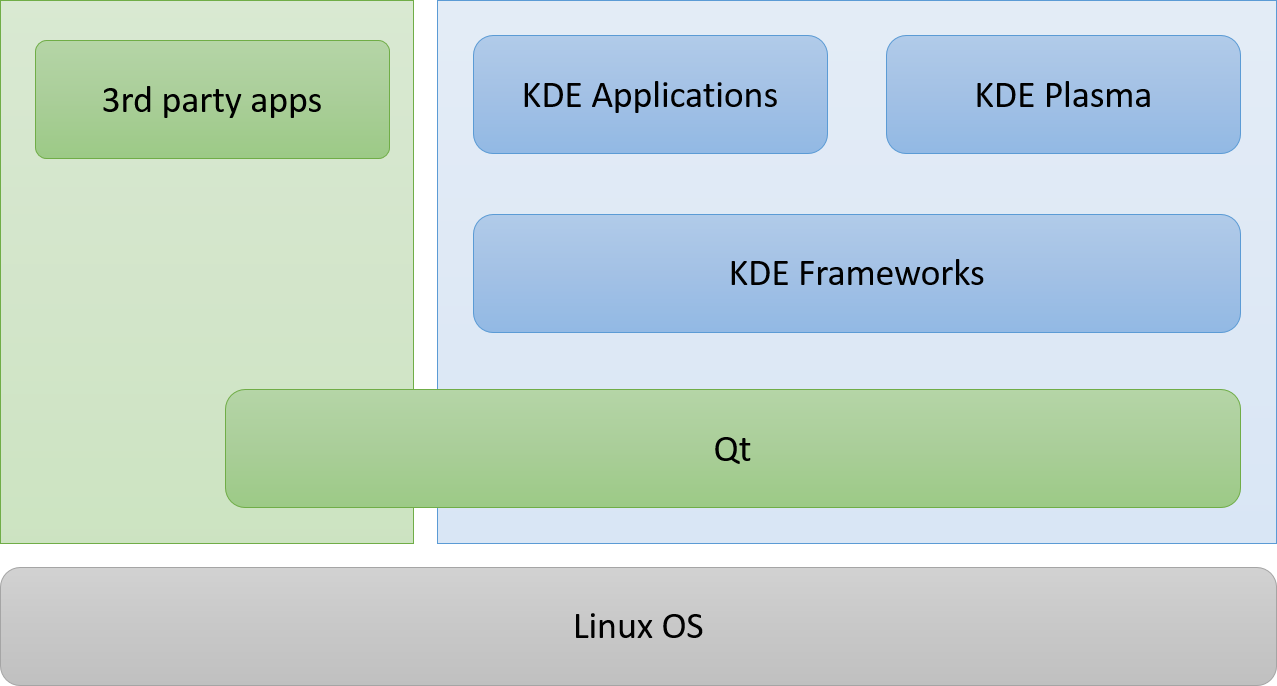
\includegraphics[width=0.8\columnwidth]{images/KDE_Aufbau.png}
\caption{KDE Übersicht}
\label{fig:kde_overview}
\end{figure}

\subsection{KDE Frameworks 5}
Das Ziel des unter der LGPL stehenden und vor allem in C++ und C entwickelten KDE Frameworks ist die Modularisierung \cite{KDEDeveloperPlatform}. Aufbauend auf das als Basis genutzte Qt 5 stellt das aktuelle KDE Frameworks 5 grundlegende und für viele Anwendungsfälle nützliche Funktionen wie z.B. extra UI Elemente, Rechtschreibprüfung, usw. zu Verfügung. KDE Frameworks stellt somit durch seine verschiedenen Bibliotheken die Basis für KDE Plasma und KDE Applications dar und vereinfacht die Entwicklung, da auf erprobte Implementierungen zurückgriffen werden kann und unnötiges für jede Software neu entwickeln verhindert wird. Das KDE Frameworks 5 besteht dazu aus rund 60 einzelnen Bibliotheken mit verschiedenen Abhängigkeiten untereinander die möglichst Plattform unabhängig gehalten sind und versuchen so wenig wie möglich zusätzliche Abhängigkeiten zu verursachen \cite{KDEFramework5TechPreview}. Für eine bessere Übersicht welche Abhängigkeiten existieren erfolgt dabei eine Einteilung ist nach "'Tier"' und "'Categorie"' die im Folgenden auch noch detaillierter vorgestellt wird \cite{KDEFramework5}. Abbildung \ref{fig:kde_frameworks} gibt einen groben Überblick für die Bestandteile der KDE Frameworks 5 und zu welchen "'Tier"' sie gehören.
%\url{https://dot.kde.org/2013/09/25/frameworks-5}
%https://www.kde.org/ https://dot.kde.org/ http://api.kde.org/

%\url{https://dot.kde.org/2014/01/07/frameworks-5-tech-preview}
%\url{https://dot.kde.org/sites/dot.kde.org/files/kf5_big_0.png}
\begin{figure*}[tb]
	\centering
	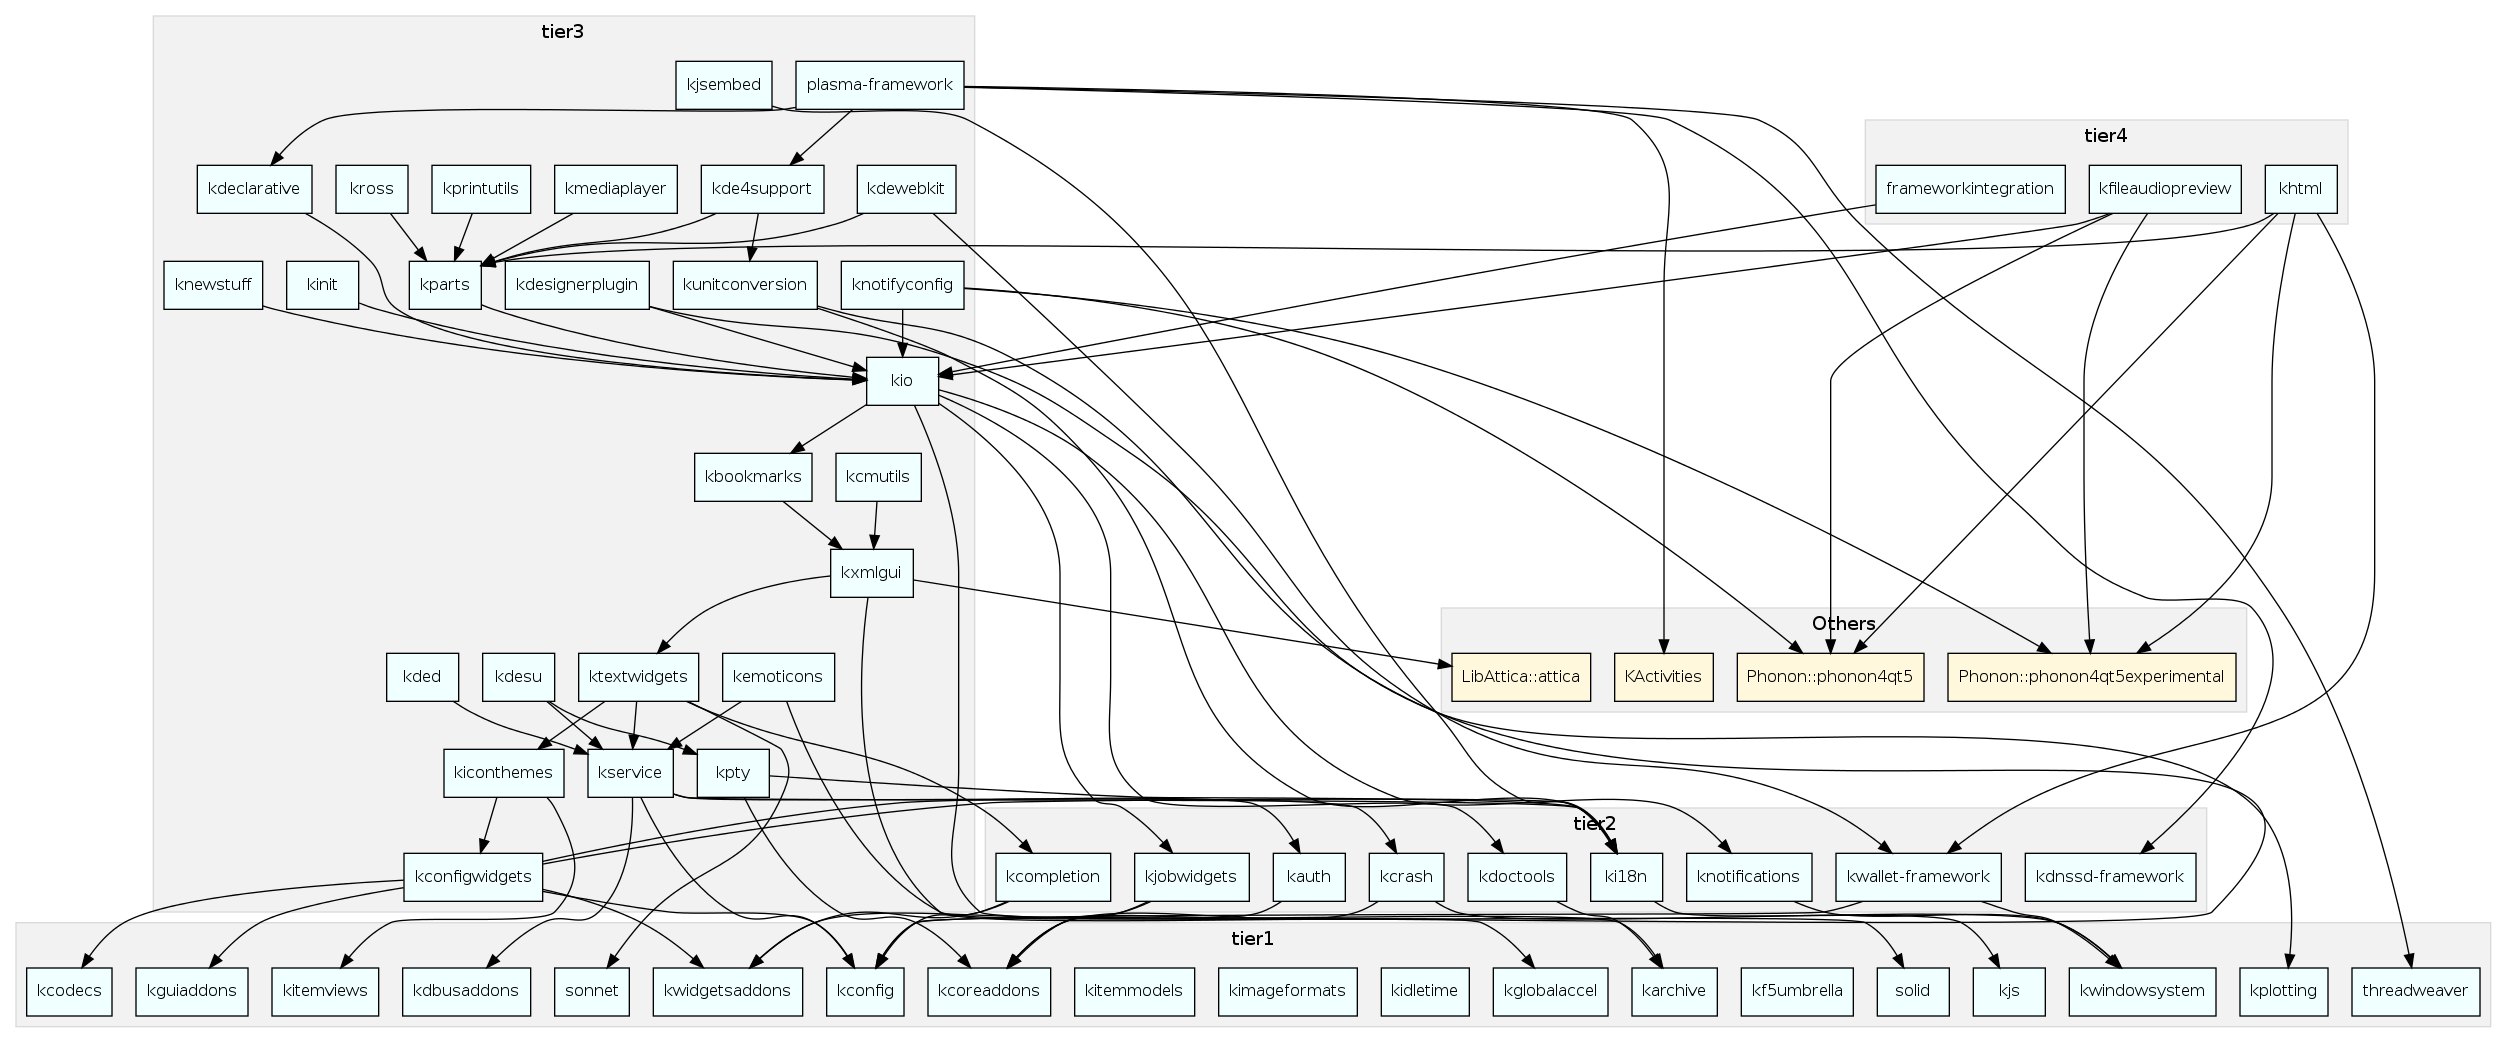
\includegraphics[width=0.85\textwidth]{images/kf5_big_0.png}
	\caption{KDE Frameworks Übersicht \cite{KDEFramework5TechPreview}}
	\label{fig:kde_frameworks}
\end{figure*}

Ziel der Aufteilung in viele einzelne in KDE Frameworks gebündelte Bibliotheken ist dabei dass es leichter möglich wird nur auf Teile der KDE Frameworks aufzubauen.
Die vielen einzelnen Bibliotheken von denen immer nur die benötigen verwendet werden ist dabei eine noch recht neue für die Architektur der Software sehr wichtige Entwicklung die erst mit KDE Frameworks 5 im Dezember 2013 eingeführt wurde. KDE Frameworks in Version 4 trug noch den Namen KDE Platfrom baute noch auf Qt 4 und war im Prinzip nur eine einzige große KDElibs Library wie sie schon in den Versionen davor existierte.
%\url{https://en.wikipedia.org/wiki/File:Evolution_and_development_of_KDE_software.svg}
\begin{figure}[h]
\centering
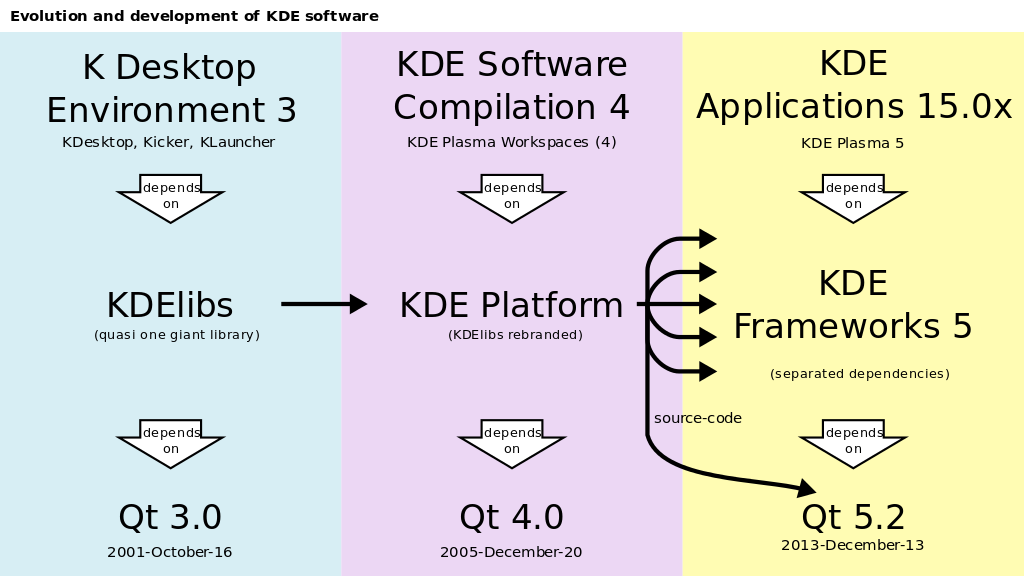
\includegraphics[width=0.8\columnwidth]{images/Evolution_and_development_of_KDE_software}
\caption{Entwicklungsgeschichte des KDE Frameworks \cite{KDEFrameworkDevelopment}}
\label{fig:Evolution_and_development_of_KDE_software}
\end{figure}

Große umbauten auf KDE Frameworks Ebene wie z.B. von Version 4 auf 5 beeinflussen allerdings alle darauf aufbauende Software weshalb verschiedene KDE Frameworks Versionen parallel von verschieden Anwendungen genutzt werden können, so dass Anwendungen die darauf aufbauen in Ruhe beim erscheinen einer neuen Version auf diese portiert werden können. Major Releases (Versionsnummer X.0) brechen dabei die Abwärtskompatibilität und steigen auch auf die nächste große Qt Version um. Minor Veröffentlichungen (X.1, X.2, ...) hingegen garanteiren Source und Binär Kompatibilität und sind meist kleine Weiterentwicklungen, Verbesserungen und vor allem Fehlerkorrekturen.

%https://www.kde.org/developerplatform/
Bekannte Frameworks aus den KDE Framworks 5 sind z.B. Sonnet eine Rechtschreib- und Grammatikprüfung, KHTML eine HTML und JS Library, Solid eine Hardware und Network Abstraktion und Phonon ein Multimedia Framework. Eine Vollständige Liste ist in der online API Dokumentation zu finden \cite{KDEDeveloperPlatform}.

Die KDE Frameworks 5 haben dabei eine klare Dependency Struktur die in "'Categorie"' und "'Tier"' einteilt \cite{KDEFramework5}. Dies hilft den Überblick zu behalten welche Abhängigkeiten der Einsatz eines bestimmten Framework mit sich bringt. In der online API Dokumentation ist deshalb auch eine Zuordnung der Farmeworks zu den Tiers verfügbar.
%\url{https://dot.kde.org/2013/09/25/frameworks-5}
%\url{http://api.kde.org/frameworks-api/frameworks5-apidocs/}

Die Einteilung "'Categories"' bezieht sich dabei wie folgt auf Laufzeit-Abhängigkeiten \cite{KDEFramework5}:
\begin{itemize}
\setlength\itemsep{0em}
\item Functional: Auf Qt aufbauend und ohne weitere Laufzeit-Abhängigkeiten z.B. KArchive, KPlotting, Threadweaver, KConfig, KCoreAddons

\item Integration: Mit optionalen Laufzeit-Abhängigkeiten für Integration bzw. Kompatibilität mit Betriebssystem/Plattform darunter z.B. Sonnet, Solid

\item Solutions: Haben gewollt Laufzeit-Abhängigkeiten um sich damit ergebende Vorteile nutzen zu können z.B. KIO, KService
\end{itemize}

Die Einteilung in "'Tiers"' bezieht sich auf die Compile-Zeit Abhängigkeiten. Von KDE Projekt wurden dazu die folgenden vier Tiers definiert \cite{KDEFramework5}:
\begin{itemize}
\setlength\itemsep{0em}
\item Tier 1: Keine Abhängigkeiten innerhalb KDE Frameworks, nur Ot und andere kleine Abhänglichkeiten  checkerso dass eine einfach Verwendung in einem Qt Projekt möglich ist. 

\item Tier 2: Dürfen auf Tier 1 Frameworks aufbauen haben aber weiterhin einfach zu verwaltende Abhängigkeiten.

\item Tier 3: Dürfen auf Tier 3 Farmworks genauso wie Tier 2 und Tier 1 Frameworks aufbauen und haben somit oft schon komplexere Abhängigkeiten.

\item Tier 4: Für Anwendungsentwickler unwichtig vor allem Frameworks zur Integration. 
\end{itemize}

Jedes Framework lässt sich somit klar einordnen. Außerdem gibt es eine vom KDE Projekt erstelle Tier/Categorie Matrix (siehe Abbildung \ref{fig:kde_matrix}) die verschieden sich damit ergebenden Kombinationen und Abhängigkeiten Zeigt.

%\url{https://dot.kde.org/sites/dot.kde.org/files/kf5_no_tier4_big.png}
\begin{figure}[h]
	\centering
	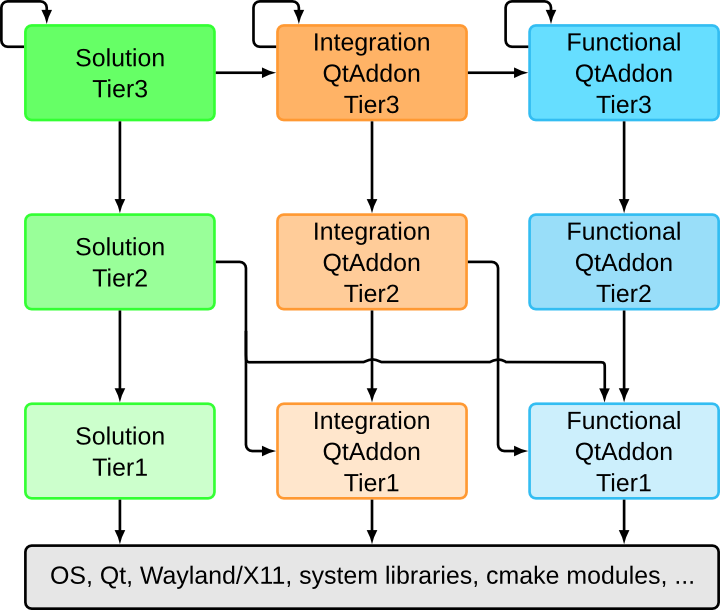
\includegraphics[width=0.9\columnwidth]{images/kf5_no_tier4_big.png}
	\caption{KDE Tier/Categorie Matrix \cite{KDEFramework5}}
	\label{fig:kde_matrix}
\end{figure}

\subsection{KDE Plasma 5} \label{plasma5}

KDE bietet zwei verschiedene Arbeitsflächen an. Jede ist dabei auf den Workflow und das entsprechend verwendete Gerät spezialisiert. So gibt es eine Arbeitsfläche für den normalen Schreibtisch-PC und Laptop-Computer und eine Arbeitsfläche für kleine Computer, wie beispielsweise Netbooks. Beide sind jeweils auf die entsprechenden Anforderungen angepasst worden. In Abbildung \ref{fig:kde_desktop} und Abbildung \ref{fig:kde_netbook} sind beide Arbeitsflächen zu sehen \cite{KDEWorkspaces}.

\begin{figure}[h]
	\centering
	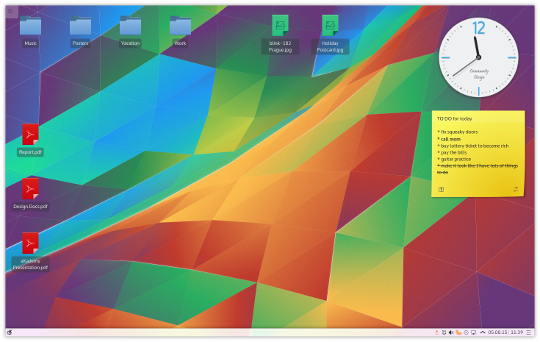
\includegraphics[width=0.9\columnwidth]{images/general-desktop.png}
	\caption{KDE Plasma Desktop Arbeitsfläche \cite{KDEWorkspaces}}
	\label{fig:kde_desktop}
\end{figure}

\begin{figure}[h]
	\centering
	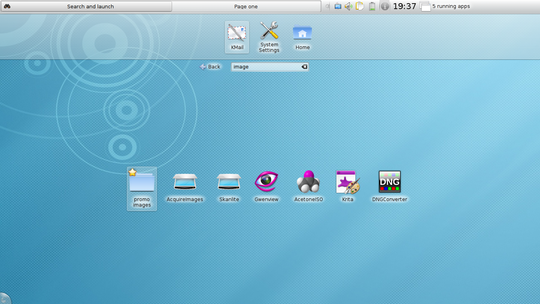
\includegraphics[width=0.9\columnwidth]{images/netbook.png}
	\caption{KDE Plasma Netbook Arbeitsfläche \cite{KDEWorkspaces}}
	\label{fig:kde_netbook}
\end{figure}


Seit KDE 4 wird die Arbeitsfläche in KDE Plasma genannt. Die neueste Version ist KDE Plasma 5 und stellt die bekannte für Linuxsysteme entwickelten Arbeitsplatzumgebung des KDE Projekts dar. Aufbauend auf Qt 5 und KDE Frameworks 5 findet die Entwicklung vor allem mit C++ und QML statt. Die Implementierung basiert auf dem Qt Graphics View Framework. Die benötigen Klassen befinden sich in der \textit{libplasma} Bibliothek. Im Folgenden werden einige Klassen vorgestellt die eine zentrale Rolle bei der Entwicklung spielen \cite{KDEPlasma}.

\begin{itemize}
	\item \textbf{Corona}: wird von \textit{QGraphicsScene} abgeleitet und bietet die Funktionalität für das Hinzufügen von \textit{Applets} und \textit{Karamba Themes}
	\item \textbf{Widget}: wird von \textit{QGraphicsItem} abgeleitet und funktioniert wie simple Elemente (zum Beispiel Icons oder auch Buttons) in der Arbeitsfläche
	\item \textbf{Applet}: wird von \textit{Widget} abgeleitet und implementiert komplexere Funktionalitäten, wie beispielsweise eine Uhr oder Systemüberwachung. Ein Beispiel für die Uhr ist in Abbildung \ref{fig:kde_desktop} zu sehen.
	\item \textbf{DataEngine}: die \textit{DataEngine} dient dazu die Daten für ein Applet bereitzustellen, damit diese angezeigt werden können. Dies gilt für alle möglichen Daten.
\end{itemize}

KDE Plasma 5 ist eine moderne Arbeitsfläche, welche alle nötigen Werkzeuge bereitstellt um effizient und produktiv arbeiten zu können. Weiterhin wird auch Wert auf das Aussehen gelegt. Mithilfe der neuen Technologien die verwendet werden, wird dieses Ziel auch erreicht. Dabei soll das Aussehen keinesfalls ablenken, sondern den Nutzer bei seiner Arbeit unterstützen. \cite{KDEPlasma}

Weiterhin soll dem Nutzer die Möglichkeit gegeben werden den Desktop nach seinem Belieben zu gestalten. Dies wird durch Widgets ermöglicht, wovon tausende online zu Verfügung stehen. Auf Wunsch kann der Nutzer auch eigene Widgets entwickeln. Hierfür stehen Tutorials zur Verfügung.


\subsection{KDE Applications 15.12}
Viele einzelne Anwendungen die zum KDE Projekt gehören werden unter den KDE Applications zusammengefasst. Das KDE Projekt teils die über hundert Anwendungen deshalb zur besseren Übersicht in folgende Kategorien \cite{KDEApps}:

\begin{itemize}
	\item \textbf{Entwicklung}: dazu gehören zum Beispiel die Apps KDevelop, KLinkStatus und Umbrello.
	\item \textbf{Bildung}: dazu gehören zum Beispiel die Apps KTouch, Step und Marble.
	\item \textbf{Spiele}: dazu gehören zum Beispiel die Apps KMines, Kolf und KLines.
	\item \textbf{Graphik}: dazu gehören zum Beispiel die Apps KSnapshot, Okular und KRuler.
	\item \textbf{Internet}: dazu gehören zum Beispiel die Apps Konqueror, KTorrent und KMail.
	\item \textbf{Multimedia}: dazu gehören zum Beispiel die Apps Amarok, KMix und KsCD.
	\item \textbf{Büro}: dazu gehören zum Beispiel die Apps Flow, Kontact und Sheets.
	\item \textbf{System}: dazu gehören zum Beispiel die Apps Dolphin, KInfoCenter und KSystemLog.
	\item \textbf{Utilities}: dazu gehören zum Beispiel die Apps Ark, Kate und KCalc.
\end{itemize}

Die verschieden Anwendungen der KDE Applications bauen, wie KDE Plasma, auf Qt und KDE Frameworks auf. Davon Abgesehen sind die einzelnen Anwendungen aber relativ unabhängig vom gesamten Projekt gehalten, weshalb auch die Architektur der einzelnen Programme oft unterschiedlich ist. 



